\documentclass{beamer}

\usetheme{boxes}

 
\usecolortheme[RGB={34,170,34}]{structure} 
\usepackage{amsmath}
\usepackage{amssymb}
\usepackage{graphics}
\usepackage{multicol}
\usepackage{color}
\usepackage[absolute,overlay]{textpos}

\usepackage{framed,color}
\definecolor{shadecolor}{rgb}{255,127,0}
\setbeamertemplate{itemize item}[circle]

\definecolor{verde}{RGB}{34,170,34}


\setbeamercolor{uppercolgreen}{fg=white,bg=verde!90}
\setbeamercolor{lowercolgreen}{fg=black,bg=verde!20}



%%%%%%%%%%%%%%%%%%%%%%%%%%%%%%%%%%%


\title[Shell Lesson]{The Shell}

\subtitle[]{EOAS Software Carpentry Workshop }
\date[Sep 2015]{September 22nd, 2015}

%------------------ the document starts here -------------------------%

\begin{document}
\bibliographystyle{plainnat}
\bibliography{bib/biblio}


%------------------ the titlepage frame-------- -------------------------%

 
\begin{frame}[plain]
  
\titlepage


\end{frame}


%-------------------------Intro--------------------------------------------%


\subsection*{Introduction}

\begin{frame}
\frametitle{Getting Started}

You need to download some files to follow this lesson. These files are found on the shell lesson website (see etherpad)

\begin{enumerate}
\item Make a new folder in your Desktop called shell-novice.
\item Download shell-novice-data.zip and move the file to this folder.
\item If it's not unzipped yet, double-click on it to unzip it. You should end up with a new folder called workshop.
\end{enumerate}
\end{frame}


\begin{frame}
\frametitle{Introduction}
\begin{block}{Learning Goals}
\begin{enumerate}

 \item   Explain how the shell relates to the keyboard, the screen, the operating system, and users' programs.
 \item   Explain when and why command-line interfaces should be used instead of graphical interfaces.

\end{enumerate}
\end{block}
\pause
\begin{block}{Why use the shell?}
\begin{itemize}
\pause
\item Connecting to supercomputers
\pause
\item Automate repetitive tasks
\pause
\item Reproducibility 
\end{itemize}
\end{block}
\end{frame}


%-------------------------FilesandDirs--------------------------------------------%

\subsection*{Files and Directories}


\begin{frame}
\frametitle{Files and Directories}
\small{
\begin{block}{Learning Goals}
\begin{enumerate}
\item    Explain the similarities and differences between a file and a directory.
\item    Translate an absolute path into a relative path and vice versa.
\item    Construct absolute and relative paths that identify specific files and directories.
\item    Explain the steps in the shell's read-run-print cycle.
\item    Identify actual command, flags, and filenames in command-line call.
\item    Demonstrate the use of tab completion, and explain its advantages.
\end{enumerate}
\end{block}}
\begin{block}{Sample Code}
\begin{multicols}{3}
\begin{itemize}
\item whoami
\item pwd
\item /
\item ls
\item ls -F
\item ls -F data
\item ls -F /data
\item cd data
\item cd ..
\item ls -F -a
\item ls north-pacific-gyre/2012-07-03
\item ls no tab
\end{itemize}
\end{multicols}
\end{block}
\end{frame}

\begin{frame}
\frametitle{Exercise}

\includegraphics[scale=0.5]{fig/filesystem-challenge.png}

If \texttt{pwd} displays \texttt{/users/backup}, and \texttt{-r} tells \texttt{ls} to display things in reverse order, what command will display:

\texttt{pnas\_sub/ pnas\_final/ original/}
\begin{enumerate}
\item ls pwd
\item ls -r -F
\item ls -r -F /users/backup
\item Either \#2 or \#3 above, but not \#1.
\end{enumerate}
\end{frame}

\begin{frame}
\frametitle{Exercise}

\includegraphics[scale=0.5]{fig/filesystem-challenge.png}

If \texttt{pwd} displays \texttt{/users/backup}, and \texttt{-r} tells \texttt{ls} to display things in reverse order, what command will display:

\texttt{pnas\_sub/ pnas\_final/ original/}
\begin{enumerate}
\item ls pwd
\item ls -r -F
\item ls -r -F /users/backup
\item \alert{Either \#2 or \#3 above, but not \#1.}
\end{enumerate}
\end{frame}


%-------------------------CreatingThings--------------------------------------------%

\subsection*{Creating Things}
\begin{frame}
\frametitle{Creating Things}
\small{
\begin{block}{Learning Goals}

\begin{enumerate}
\item    Create a directory hierarchy that matches a given diagram.
\item    Create files in that hierarchy using an editor or by copying and renaming existing files.
\item    Display the contents of a directory using the command line.
\item    Delete specified files and/or directories.
\end{enumerate}
\end{block}
\begin{block}{Sample Code}
\begin{multicols}{2}
\begin{itemize}
\item mkdir thesis
\item cd thesis
\item nano draft.txt
\item rm draft.txt
\item rm thesis
\item rmdir thesis
\item rm -r thesis
\item mv thesis/draft.txt thesis/quotes.txt
\item mv thesis/quotes.txt .
\item cp quotes.txt thesis/quotations.txt
\end{itemize}
\end{multicols}
\end{block}}
\end{frame}


\begin{frame}[fragile]
\frametitle{Exercise}
Jamie is working on a project and she sees that her files aren’t very well organized:
\begin{verbatim}
$ ls -F
analyzed/  fructose.dat    raw/   sucrose.dat
\end{verbatim}
The fructose.dat and sucrose.dat files contain output from her data analysis. 
What command(s) could you run so that the commands below will produce the output shown? 
\begin{verbatim}
$ ls
analyzed   raw
$ ls analyzed
fructose.dat   sucrose.dat
\end{verbatim}
\end{frame}

\begin{frame}[fragile]
\frametitle{Exercise}
Jamie is working on a project and she sees that her files aren’t very well organized:
\begin{verbatim}
$ ls -F
analyzed/  fructose.dat    raw/   sucrose.dat
\end{verbatim}
The fructose.dat and sucrose.dat files contain output from her data analysis. 
What command(s) could you run so that the commands below will produce the output shown? 
\begin{verbatim}
$ ls
analyzed   raw
$ ls analyzed
fructose.dat   sucrose.dat
\end{verbatim}

\begin{block}{Solution}
\begin{verbatim}
$ mv fructose.dat analyzed/fructose.dat
$ mv sucrose.dat analyzed/sucrose.dat
\end{verbatim}
\end{block}
\end{frame}

%-------------------------Pipes--------------------------------------------%

\subsection*{PipesAndFilters}
\begin{frame}
\frametitle{Pipes and Filters}
\small{
\begin{block}{Learning Goals}
\begin{enumerate}
\item    Redirect a command's output to a file.
\item    Process a file instead of keyboard input using redirection.
\item    Construct command pipelines with two or more stages.
\item    Explain what usually happens if a program or pipeline isn't given any input to process.
\item    Explain Unix's "small pieces, loosely joined" philosophy.
\end{enumerate}
\end{block}

\begin{multicols}{2}
\begin{itemize}
\item cd molecules
\item wc *.pdb
\item wc -l
\item wc -l *.pdb $>$ lengths
\item cat lengths
\item sort lengths
\item sort lengths $>$ sorted-lengths
\item head -1 sorted-lengths
\item sort lengths $|$ head -1
\item wc -l *.txt
\item wc -l *.txt $|$ sort $|$ head -5
\item ls *Z.txt
\end{itemize}
\end{multicols}}
\end{frame}


\begin{frame}
\frametitle{Exercise}
In our current directory, we want to find the 3 files which have the least number of lines. Which command listed below would work?

\begin{enumerate}
\item wc -l * $>$ sort -n $>$ head -3
\item wc -l * $|$ sort -n $|$ head 1-3
\item wc -l * $|$ head -3 $|$ sort -n
\item wc -l * $|$ sort -n $|$ head -3
\end{enumerate}
\end{frame}

\begin{frame}
\frametitle{Exercise}
In our current directory, we want to find the 3 files which have the least number of lines. Which command listed below would work?

\begin{enumerate}
\item wc -l * $>$ sort -n $>$ head -3
\item wc -l * $|$ sort -n $|$ head 1-3
\item wc -l * $|$ head -3 $|$ sort -n
\alert{\item wc -l * $|$ sort -n $|$ head -3}
\end{enumerate}
\end{frame}


%-------------------------- Loops-Intro------------------------------------------%

\begin{frame}{Loops}

\begin{figure}[htbp]
   \centering
   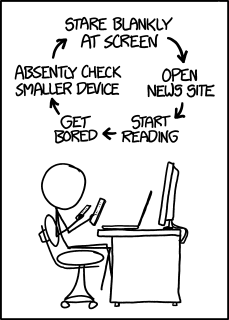
\includegraphics[width=0.45\textwidth]{figs_slides/loops.png} 
\end{figure}

\begin{textblock*}{7cm}(6.0cm,9.0cm)
		\centering
			\tiny{https://xkcd.com/1411/ }
\end{textblock*}

\end{frame}
%-------------------------- objectives ------------------------------------------%

\begin{frame}{Loops}
\begin{itemize}
    \item{Write a loop that applies one or more commands separately to each file in a set of files.}
    \item{Trace the values taken on by a loop variable during execution of the loop.}
    \item{Explain the difference between a variable's name and its value.}
    \item{Explain why spaces and some punctuation characters shouldn't be used in file names.}
    \item{Demonstrate how to see what commands have recently been executed.}
    \item{Re-run recently executed commands without retyping them.}
    \end{itemize}
\end{frame}


%-------------------------- Challenge 01 ------------------------------------------%

\begin{frame}{Variables in loops}
Suppose that \texttt{ls} initially displays:
\vspace{0.7cm}
\begin{beamerboxesrounded}[upper=uppercolgreen,lower=lowercolgreen,shadow=false]{}
fructose.dat      glucose.dat       sucrose.dat
\end{beamerboxesrounded}

What is the output of:
\vspace{0.7cm}
\begin{beamerboxesrounded}[upper=uppercolgreen,lower=lowercolgreen,shadow=false]{}
\texttt{for datafile in *.dat}

\texttt{do}

\texttt{	ls *.dat}

\texttt{done}
\end{beamerboxesrounded}

\end{frame}

%-------------------------- Challenge 01 - SOLUTION ------------------------------------------%

\begin{frame}{Variables in loops}
Suppose that \texttt{ls} initially displays:
\vspace{0.7cm}
\begin{beamerboxesrounded}[upper=uppercolgreen,lower=lowercolgreen,shadow=false]{}
fructose.dat      glucose.dat       sucrose.dat
\end{beamerboxesrounded}

What is the output of:
\vspace{0.7cm}
\begin{beamerboxesrounded}[upper=uppercolgreen,lower=lowercolgreen,shadow=false]{}
\texttt{for datafile in *.dat}

\texttt{do}

\texttt{	ls *.dat}

\texttt{done}
\end{beamerboxesrounded}

\alert{ANSWER:\\ }
fructose.dat      glucose.dat       sucrose.dat\\
fructose.dat      glucose.dat       sucrose.dat\\
fructose.dat      glucose.dat       sucrose.dat\\

\end{frame}


%-------------------------- Challenge 02 ------------------------------------------%

\begin{frame}{Saving to a file in a loop }
In the same directory, what is the effect of this loop?

\begin{beamerboxesrounded}[upper=uppercolgreen,lower=lowercolgreen,shadow=false]{}
\texttt{for sugar in *.dat}

\texttt{do}

\texttt{	echo \$sugar}

\texttt{	cat \$sugar > xylose.dat}

\texttt{done}
\end{beamerboxesrounded}

\small{
\begin{enumerate}
\item{Prints \texttt{fructose.dat, glucose.dat, and sucrose.dat}, and the text from \texttt{sucrose.dat} will be saved to a file called \texttt{xylose.dat}.}
\item{Prints \texttt{fructose.dat, glucose.dat, and sucrose.dat}, and the text from all three files would be concatenated and saved to a file called \texttt{xylose.dat}.}
\item{Prints \texttt{fructose.dat, glucose.dat, sucrose.dat, and xylose.dat}, and the text from \texttt{sucrose.dat}  will be saved to a file called \texttt{xylose.dat}.}
\item{None of the above}
\end{enumerate}}


\end{frame}

%-------------------------- Challenge 02 - SOLUTION------------------------------------------%

\begin{frame}{Saving to a file in a loop }
In the same directory, what is the effect of this loop?

\begin{beamerboxesrounded}[upper=uppercolgreen,lower=lowercolgreen,shadow=false]{}
\texttt{for sugar in *.dat}

\texttt{do}

\texttt{	echo \$sugar}

\texttt{	cat \$sugar > xylose.dat}

\texttt{done}
\end{beamerboxesrounded}

\small{
\begin{enumerate}
\alert{\item{Prints \texttt{fructose.dat, glucose.dat, and sucrose.dat}, and the text from \texttt{sucrose.dat} will be saved to a file called \texttt{xylose.dat}.}}
\item{Prints \texttt{fructose.dat, glucose.dat, and sucrose.dat}, and the text from all three files would be concatenated and saved to a file called \texttt{xylose.dat}.}
\item{Prints \texttt{fructose.dat, glucose.dat, sucrose.dat, and xylose.dat}, and the text from \texttt{sucrose.dat}  will be saved to a file called \texttt{xylose.dat}.}
\item{None of the above}
\end{enumerate}}


\end{frame}

%-------------------------- Scripts ------------------------------------------%
\begin{frame}{Scripts}
\begin{enumerate}
   \item{ Write a shell script that runs a command or series of commands for a fixed set of files.}
   \item{  Run a shell script from the command line.}
   \item{ Write a shell script that operates on a set of files defined by the user on the command line.}
   \item{  Create pipelines that include user-written shell scripts.}
\end{enumerate}
\end{frame}

%-------------------------- Challenge 01------------------------------------------%

\begin{frame}{}
In the \texttt{molecules} directory, you have a shell script called \texttt{script.sh} containing the following commands:
\begin{beamerboxesrounded}[upper=uppercolgreen,lower=lowercolgreen,shadow=false]{}
\small{\texttt{head \$2 \$1 \\ tail \$3 \$1}}
\end{beamerboxesrounded}

While you are in the molecules directory, you type the following command:

\begin{beamerboxesrounded}[upper=uppercolgreen,lower=lowercolgreen,shadow=false]{}
\small{\texttt{bash script.sh `*.pdb' -1 -1}}
\end{beamerboxesrounded}

Which of the following outputs would you expect to see?

\begin{enumerate}
\item{All of the lines between the first and the last lines of each file ending in *.pdb in the molecules directory}
    \item{The first and the last line of each file ending in *.pdb in the molecules directory}
    \item{The first and the last line of each file in the molecules directory}
    \item{An error because of the quotes around *.pdb}
\end{enumerate}


\end{frame}
%-------------------------- Challenge 01 Sol------------------------------------------%

\begin{frame}{}
In the \texttt{molecules} directory, you have a shell script called \texttt{script.sh} containing the following commands:
\begin{beamerboxesrounded}[upper=uppercolgreen,lower=lowercolgreen,shadow=false]{}
\small{\texttt{head \$2 \$1 \\ tail \$3 \$1}}
\end{beamerboxesrounded}

While you are in the molecules directory, you type the following command:

\begin{beamerboxesrounded}[upper=uppercolgreen,lower=lowercolgreen,shadow=false]{}
\small{\texttt{bash script.sh `*.pdb' -1 -1}}
\end{beamerboxesrounded}

Which of the following outputs would you expect to see?

\begin{enumerate}
\item{All of the lines between the first and the last lines of each file ending in *.pdb in the molecules directory}
    \alert{\item{The first and the last line of each file ending in *.pdb in the molecules directory}}
    \item{The first and the last line of each file in the molecules directory}
    \item{An error because of the quotes around *.pdb}
\end{enumerate}


\end{frame}

%-------------------------- Challenge 02------------------------------------------%

\begin{frame}{Why record commands in the history before running them?}
If you run the command:

\vspace{0.5cm}


\begin{beamerboxesrounded}[upper=uppercolgreen,lower=lowercolgreen,shadow=false]{}
\small{\texttt{\$ history | tail -5 > recent.sh}}
\end{beamerboxesrounded}

\vspace{0.5cm}

he last command in the file is the \texttt{history} command itself, i.e., the shell has added \texttt{history} to the command log before actually running it. In fact, the shell always adds commands to the log before running them. Why do you think it does this?
\end{frame}


%-------------------------- Challenge 03------------------------------------------%

\begin{frame}{Script reading comprehension}

Joel's data directory contains three files: \texttt{fructose.dat, glucose.dat}, and \texttt{sucrose.dat}. Explain what a script called \texttt{example.sh} would do when run as bash \texttt{example.sh *.dat} if it contained the following lines:
\vspace{0.5cm}


\begin{beamerboxesrounded}[upper=uppercolgreen,lower=lowercolgreen,shadow=false]{}
\small{\texttt{\# Script 1\\
echo *.*}}
\end{beamerboxesrounded}

\begin{beamerboxesrounded}[upper=uppercolgreen,lower=lowercolgreen,shadow=false]{}
\small{\texttt{\# Script 2\\
for filename in \$1 \$2 \$3\\
do\\}
\texttt{         cat \$filename\\}
\texttt{done\\}}
\end{beamerboxesrounded}

\begin{beamerboxesrounded}[upper=uppercolgreen,lower=lowercolgreen,shadow=false]{}
\small{\texttt{\# Script 3\\
echo \$*.dat}}
\end{beamerboxesrounded}


\end{frame}

%-------------------------- Challenge 03 - SOL------------------------------------------%

\begin{frame}{Script reading comprehension}

Joel's data directory contains three files: \texttt{fructose.dat, glucose.dat}, and \texttt{sucrose.dat}. Explain what a script called \texttt{example.sh} would do when run as bash \texttt{example.sh *.dat} if it contained the following lines:
\vspace{0.5cm}


\begin{beamerboxesrounded}[upper=uppercolgreen,lower=lowercolgreen,shadow=false]{}
\small{\texttt{\# Script 1\\
echo *.*}}
\end{beamerboxesrounded}

\alert{ANSWER:}

Prints 

\texttt{example.sh fructose.dat   glucose.dat    sucrose.dat}   

\end{frame}

%-------------------------- Challenge 3 - Sol------------------------------------------%

\begin{frame}{Script reading comprehension}

Joel's data directory contains three files: \texttt{fructose.dat, glucose.dat}, and \texttt{sucrose.dat}. Explain what a script called \texttt{example.sh} would do when run as bash \texttt{example.sh *.dat} if it contained the following lines:
\vspace{0.5cm}

\begin{beamerboxesrounded}[upper=uppercolgreen,lower=lowercolgreen,shadow=false]{}
\small{\texttt{\# Script 2\\
for filename in \$1 \$2 \$3\\
do\\}
\texttt{         cat \$filename\\}
\texttt{done\\}}
\end{beamerboxesrounded}

\alert{ANSWER:}

Shows contents of fructose.dat, glucose.dat, and sucrose.dat

\end{frame}

%-------------------------- Challenge 03 - SOL------------------------------------------%

\begin{frame}{Script reading comprehension}

Joel's data directory contains three files: \texttt{fructose.dat, glucose.dat}, and \texttt{sucrose.dat}. Explain what a script called \texttt{example.sh} would do when run as bash \texttt{example.sh *.dat} if it contained the following lines:
\vspace{0.5cm}

\begin{beamerboxesrounded}[upper=uppercolgreen,lower=lowercolgreen,shadow=false]{}
\small{\texttt{\# Script 3\\
echo \$*.dat}}
\end{beamerboxesrounded}

\alert{ANSWER:}

Prints

\texttt{fructose.dat glucose.dat sucrose.dat.dat}

\end{frame}


%-------------------------- Finding things ------------------------------------------%

\begin{frame}{Finding things}

\begin{enumerate}
    \item{Use \texttt{grep} to select lines from text files that match simple patterns.}
    \item{Use \texttt{find} to find files whose names match simple patterns.}
    \item{Use the output of one command as the command-line parameters to another command.}
    \item{Explain what is meant by `text' and `binary' files, and why many common tools don't handle the latter well.}
\end{enumerate}


\end{frame}

%-------------------------- Challenge 01------------------------------------------%

\begin{frame}{\texttt{find} pipeline reading comprehension}

Write a short explanatory comment for the following shell script:
\vspace{0.5cm}

\begin{beamerboxesrounded}[upper=uppercolgreen,lower=lowercolgreen,shadow=false]{}
\texttt{find . -name `*.dat' -print | wc -l | sort -n}
\end{beamerboxesrounded}


\end{frame}

%-------------------------- Challenge 02------------------------------------------%

\begin{frame}{Matching \texttt{ose.dat} but not \texttt{temp}}

The \texttt{-v} flag to \texttt{grep} inverts pattern matching, so that only lines which do not match the pattern are printed. Given that, which of the following commands will find all files in \texttt{/data} whose names end in \texttt{ose.dat} (e.g., \texttt{sucrose.dat} or \texttt{maltose.dat}), but do not contain the word \texttt{temp}?


\begin{enumerate}

\item{\texttt{find /data -name `*.dat' -print | grep ose | grep -v temp}}
\item{\texttt{find /data -name \text{ose.dat} -print | grep -v temp}}
\item{\texttt{grep -v "temp" \$(find /data -name `*ose.dat' -print)}}
\item{None of the above.}

\end{enumerate}

\end{frame}

%-------------------------- Challenge 02 - SOL------------------------------------------%

\begin{frame}{Matching \texttt{ose.dat} but not \texttt{temp}}

The \texttt{-v} flag to \texttt{grep} inverts pattern matching, so that only lines which do not match the pattern are printed. Given that, which of the following commands will find all files in \texttt{/data} whose names end in \texttt{ose.dat} (e.g., \texttt{sucrose.dat} or \texttt{maltose.dat}), but do not contain the word \texttt{temp}?


\begin{enumerate}

\item{\texttt{find /data -name `*.dat' -print | grep ose | grep -v temp}}
\item{\texttt{find /data -name \text{ose.dat} -print | grep -v temp}}
\alert{\item{\texttt{grep -v "temp" \$(find /data -name `*ose.dat' -print)}}}
\item{None of the above.}

\end{enumerate}

\end{frame}

%-------------------------- the document ends here ----------------------------------%

\end{document}
